% Options for packages loaded elsewhere
\PassOptionsToPackage{unicode}{hyperref}
\PassOptionsToPackage{hyphens}{url}
%
\documentclass[
  8pt,
  ignorenonframetext,
]{beamer}
\usepackage{pgfpages}
\setbeamertemplate{caption}[numbered]
\setbeamertemplate{caption label separator}{: }
\setbeamercolor{caption name}{fg=normal text.fg}
\beamertemplatenavigationsymbolsempty
% Prevent slide breaks in the middle of a paragraph
\widowpenalties 1 10000
\raggedbottom
\setbeamertemplate{part page}{
  \centering
  \begin{beamercolorbox}[sep=16pt,center]{part title}
    \usebeamerfont{part title}\insertpart\par
  \end{beamercolorbox}
}
\setbeamertemplate{section page}{
  \centering
  \begin{beamercolorbox}[sep=12pt,center]{part title}
    \usebeamerfont{section title}\insertsection\par
  \end{beamercolorbox}
}
\setbeamertemplate{subsection page}{
  \centering
  \begin{beamercolorbox}[sep=8pt,center]{part title}
    \usebeamerfont{subsection title}\insertsubsection\par
  \end{beamercolorbox}
}
\AtBeginPart{
  \frame{\partpage}
}
\AtBeginSection{
  \ifbibliography
  \else
    \frame{\sectionpage}
  \fi
}
\AtBeginSubsection{
  \frame{\subsectionpage}
}
\usepackage{amsmath,amssymb}
\usepackage{lmodern}
\usepackage{iftex}
\ifPDFTeX
  \usepackage[T1]{fontenc}
  \usepackage[utf8]{inputenc}
  \usepackage{textcomp} % provide euro and other symbols
\else % if luatex or xetex
  \usepackage{unicode-math}
  \defaultfontfeatures{Scale=MatchLowercase}
  \defaultfontfeatures[\rmfamily]{Ligatures=TeX,Scale=1}
\fi
% Use upquote if available, for straight quotes in verbatim environments
\IfFileExists{upquote.sty}{\usepackage{upquote}}{}
\IfFileExists{microtype.sty}{% use microtype if available
  \usepackage[]{microtype}
  \UseMicrotypeSet[protrusion]{basicmath} % disable protrusion for tt fonts
}{}
\makeatletter
\@ifundefined{KOMAClassName}{% if non-KOMA class
  \IfFileExists{parskip.sty}{%
    \usepackage{parskip}
  }{% else
    \setlength{\parindent}{0pt}
    \setlength{\parskip}{6pt plus 2pt minus 1pt}}
}{% if KOMA class
  \KOMAoptions{parskip=half}}
\makeatother
\usepackage{xcolor}
\newif\ifbibliography
\usepackage{color}
\usepackage{fancyvrb}
\newcommand{\VerbBar}{|}
\newcommand{\VERB}{\Verb[commandchars=\\\{\}]}
\DefineVerbatimEnvironment{Highlighting}{Verbatim}{commandchars=\\\{\}}
% Add ',fontsize=\small' for more characters per line
\usepackage{framed}
\definecolor{shadecolor}{RGB}{248,248,248}
\newenvironment{Shaded}{\begin{snugshade}}{\end{snugshade}}
\newcommand{\AlertTok}[1]{\textcolor[rgb]{0.94,0.16,0.16}{#1}}
\newcommand{\AnnotationTok}[1]{\textcolor[rgb]{0.56,0.35,0.01}{\textbf{\textit{#1}}}}
\newcommand{\AttributeTok}[1]{\textcolor[rgb]{0.77,0.63,0.00}{#1}}
\newcommand{\BaseNTok}[1]{\textcolor[rgb]{0.00,0.00,0.81}{#1}}
\newcommand{\BuiltInTok}[1]{#1}
\newcommand{\CharTok}[1]{\textcolor[rgb]{0.31,0.60,0.02}{#1}}
\newcommand{\CommentTok}[1]{\textcolor[rgb]{0.56,0.35,0.01}{\textit{#1}}}
\newcommand{\CommentVarTok}[1]{\textcolor[rgb]{0.56,0.35,0.01}{\textbf{\textit{#1}}}}
\newcommand{\ConstantTok}[1]{\textcolor[rgb]{0.00,0.00,0.00}{#1}}
\newcommand{\ControlFlowTok}[1]{\textcolor[rgb]{0.13,0.29,0.53}{\textbf{#1}}}
\newcommand{\DataTypeTok}[1]{\textcolor[rgb]{0.13,0.29,0.53}{#1}}
\newcommand{\DecValTok}[1]{\textcolor[rgb]{0.00,0.00,0.81}{#1}}
\newcommand{\DocumentationTok}[1]{\textcolor[rgb]{0.56,0.35,0.01}{\textbf{\textit{#1}}}}
\newcommand{\ErrorTok}[1]{\textcolor[rgb]{0.64,0.00,0.00}{\textbf{#1}}}
\newcommand{\ExtensionTok}[1]{#1}
\newcommand{\FloatTok}[1]{\textcolor[rgb]{0.00,0.00,0.81}{#1}}
\newcommand{\FunctionTok}[1]{\textcolor[rgb]{0.00,0.00,0.00}{#1}}
\newcommand{\ImportTok}[1]{#1}
\newcommand{\InformationTok}[1]{\textcolor[rgb]{0.56,0.35,0.01}{\textbf{\textit{#1}}}}
\newcommand{\KeywordTok}[1]{\textcolor[rgb]{0.13,0.29,0.53}{\textbf{#1}}}
\newcommand{\NormalTok}[1]{#1}
\newcommand{\OperatorTok}[1]{\textcolor[rgb]{0.81,0.36,0.00}{\textbf{#1}}}
\newcommand{\OtherTok}[1]{\textcolor[rgb]{0.56,0.35,0.01}{#1}}
\newcommand{\PreprocessorTok}[1]{\textcolor[rgb]{0.56,0.35,0.01}{\textit{#1}}}
\newcommand{\RegionMarkerTok}[1]{#1}
\newcommand{\SpecialCharTok}[1]{\textcolor[rgb]{0.00,0.00,0.00}{#1}}
\newcommand{\SpecialStringTok}[1]{\textcolor[rgb]{0.31,0.60,0.02}{#1}}
\newcommand{\StringTok}[1]{\textcolor[rgb]{0.31,0.60,0.02}{#1}}
\newcommand{\VariableTok}[1]{\textcolor[rgb]{0.00,0.00,0.00}{#1}}
\newcommand{\VerbatimStringTok}[1]{\textcolor[rgb]{0.31,0.60,0.02}{#1}}
\newcommand{\WarningTok}[1]{\textcolor[rgb]{0.56,0.35,0.01}{\textbf{\textit{#1}}}}
\setlength{\emergencystretch}{3em} % prevent overfull lines
\providecommand{\tightlist}{%
  \setlength{\itemsep}{0pt}\setlength{\parskip}{0pt}}
\setcounter{secnumdepth}{-\maxdimen} % remove section numbering
% type setting
% ------------------------------------------------------------------------------
\usepackage[german]{babel}     

% fonts
% ------------------------------------------------------------------------------
\usefonttheme{professionalfonts}

% slide title and horizontal line
% ------------------------------------------------------------------------------
\setbeamertemplate{frametitle}{%
    \vskip-30pt \color{black}\large%
    \begin{minipage}[b][23pt]{120mm}%
    \flushleft\insertframetitle%
    \end{minipage}%
}

\setbeamertemplate{headline}										
{
\vskip10pt\hfill\hspace{3.5mm} 										 
\vskip15pt\color{black}\rule{\textwidth}{0.4pt} 					 
}

% slide number
% ---------------------------------------------------------------
\setbeamertemplate{navigation symbols}{}
\setbeamertemplate{footline}
{
\vskip5pt
\vskip2pt
\makebox[123mm]{\hspace{7.5mm}
\hfill Multivariate Datenanalyse $\vert$ 
\copyright $ $ 2023 Dirk Ostwald CC BY-SA 4.0 $\vert$ 
Folie \insertframenumber}
\vskip4pt
}

% block color scheme
% ------------------------------------------------------------------------------
% colors
\definecolor{white}{RGB}{255,255,255}
\definecolor{grey}{RGB}{235,235,235}
\definecolor{lightgrey}{RGB}{245,245,245}
\definecolor{LightBlue}{RGB}{220,220,255}
\definecolor{darkblue}{RGB}{51, 51, 153}

% definitions and theorems
\setbeamercolor{block title}{fg = black, bg = grey}
\setbeamercolor{block body}{fg = black, bg = lightgrey}

% general line spacing 
% ------------------------------------------------------------------------------
\linespread{1.3}

% local line spacing
% ------------------------------------------------------------------------------
\usepackage{setspace}

% colors
% -----------------------------------------------------------------------------
\usepackage{color}

% justified text
% ------------------------------------------------------------------------------
\usepackage{ragged2e}
\usepackage{etoolbox}
\apptocmd{\frame}{}{\justifying}{}

% bullet point lists
% -----------------------------------------------------------------------------
\setbeamertemplate{itemize item}[circle]
\setbeamertemplate{itemize subitem}[circle]
\setbeamertemplate{itemize subsubitem}[circle]
\setbeamercolor{itemize item}{fg = black}
\setbeamercolor{itemize subitem}{fg = black}
\setbeamercolor{itemize subsubitem}{fg = black}
\setbeamercolor{enumerate item}{fg = black}
\setbeamercolor{enumerate subitem}{fg = black}
\setbeamercolor{enumerate subsubitem}{fg = black}
\setbeamerfont{itemize/enumerate body}{}
\setbeamerfont{itemize/enumerate subbody}{size = \normalsize}
\setbeamerfont{itemize/enumerate subsubbody}{size = \normalsize}

% color links
% ------------------------------------------------------------------------------
\usepackage{hyperref}
\definecolor{urls}{RGB}{204,0,0}
\hypersetup{colorlinks, citecolor = darkblue, urlcolor = urls}


% additional math commands
% ------------------------------------------------------------------------------
\usepackage{bm}                                
\usepackage{mathtools}                        
\newcommand{\niton}{\not\owns}
\DeclareMathOperator*{\intinf}{\int_{-\infty}^{\infty}}
\DeclareMathOperator*{\ups}{\upsilon}

% text highlighting
% ------------------------------------------------------------------------------
\usepackage{soul}
\makeatletter
\let\HL\hl
\renewcommand\hl{%
  \let\set@color\beamerorig@set@color
  \let\reset@color\beamerorig@reset@color
  \HL}
\makeatother

% equation highlighting
% -----------------------------------------------------------------------------
\newcommand{\highlight}[2][yellow]{\mathchoice%
  {\colorbox{#1}{$\displaystyle#2$}}%
  {\colorbox{#1}{$\textstyle#2$}}%
  {\colorbox{#1}{$\scriptstyle#2$}}%
  {\colorbox{#1}{$\scriptscriptstyle#2$}}}%

\ifLuaTeX
  \usepackage{selnolig}  % disable illegal ligatures
\fi
\IfFileExists{bookmark.sty}{\usepackage{bookmark}}{\usepackage{hyperref}}
\IfFileExists{xurl.sty}{\usepackage{xurl}}{} % add URL line breaks if available
\urlstyle{same} % disable monospaced font for URLs
\hypersetup{
  hidelinks,
  pdfcreator={LaTeX via pandoc}}

\author{}
\date{\vspace{-2.5em}}

\begin{document}

\begin{frame}[plain]{}
\protect\hypertarget{section}{}
\center

\begin{center}
\includegraphics[width=0.2\linewidth]{5_Abbildungen/mvda_5_otto} \end{center}

\vspace{2mm}

\Huge

Multivariate Datenanalyse \vspace{6mm}

\large

MSc Psychologie WiSe 2022/23

\vspace{6mm}
\large

Prof.~Dr.~Dirk Ostwald
\end{frame}

\begin{frame}[plain]{}
\protect\hypertarget{section-1}{}
\vfill
\center
\huge

\textcolor{black}{(5) Multivariate Wahrscheinlichkeitstheorie} \vfill
\end{frame}

\begin{frame}{}
\protect\hypertarget{section-2}{}
\large
\setstretch{2.5}
\vfill

Vorbemerkungen

Multivariate Verteilungen

Marginalverteilungen und Bedingte Verteilungen

Erwartungswert, Kovarianzmatrizen und Korrelationsmatrizen

Selbstkontrollfragen \vfill
\end{frame}

\begin{frame}{}
\protect\hypertarget{section-3}{}
\large
\setstretch{2.5}
\vfill

\textbf{Vorbemerkungen}

Multivariate Verteilungen

Marginalverteilungen und Bedingte Verteilungen

Erwartungswert, Kovarianzmatrizen und Korrelationsmatrizen

Selbstkontrollfragen \vfill
\end{frame}

\begin{frame}{Vorbemerkungen}
\protect\hypertarget{vorbemerkungen}{}
\vspace{2mm}

\textcolor{darkblue}{Modul A1/A3 Forschungsmethoden: Multivariate Verfahren | Themen}
\vspace{2mm}

\center
\footnotesize
\renewcommand{\arraystretch}{1.1}
\begin{tabular}{lll}
Datum        & Einheit                          & Thema                                               \\\hline
14.10.2022   & Grundlagen                       & (1) Einführung                                      \\
21.10.2022   & Grundlagen                       & (2) Vektoren                                \\
28.10.2022   & Grundlagen                       & (3) Matrizen                                \\
04.11.2022   & Grundlagen                       & (4) Eigenanalyse                            \\
11.11.2022   & Grundlagen                       & (5) Multivariate Wahrscheinlichkeitstheorie \\
18.11.2022   & Grundlagen                       & (6) Multivariate Normalverteilungen         \\
25.11.2022   & Frequentistische Inferenz        & (7) Kanonische Korrelation                  \\
02.12.2022   & Frequentistische Inferenz        & (8) T$^2$-Tests                             \\
09.12.2022   & Frequentistische Inferenz        & (9) Einfaktorielle MANOVA                   \\
16.12.2022   & Latente Variablenmodelle         & (10) Hauptkomponentenanalyse                \\
             & \textcolor{gray}{Weihnachtspause}                                              \\
13.01.2023   & Latente Variablenmodelle         & (12) Lineare Normalverteilungsmodelle       \\
20.01.2023   & Latente Variablenmodelle         & (13) Konfirmatorische Faktorenanalyse       \\
27.01.2023   & Latente Variablenmodelle         & (14) Exploratorische Faktorenanalyse        \\\hline
\end{tabular}
\end{frame}

\begin{frame}{Vorbemerkungen}
\protect\hypertarget{vorbemerkungen-1}{}
\vspace{2mm}

\begin{center}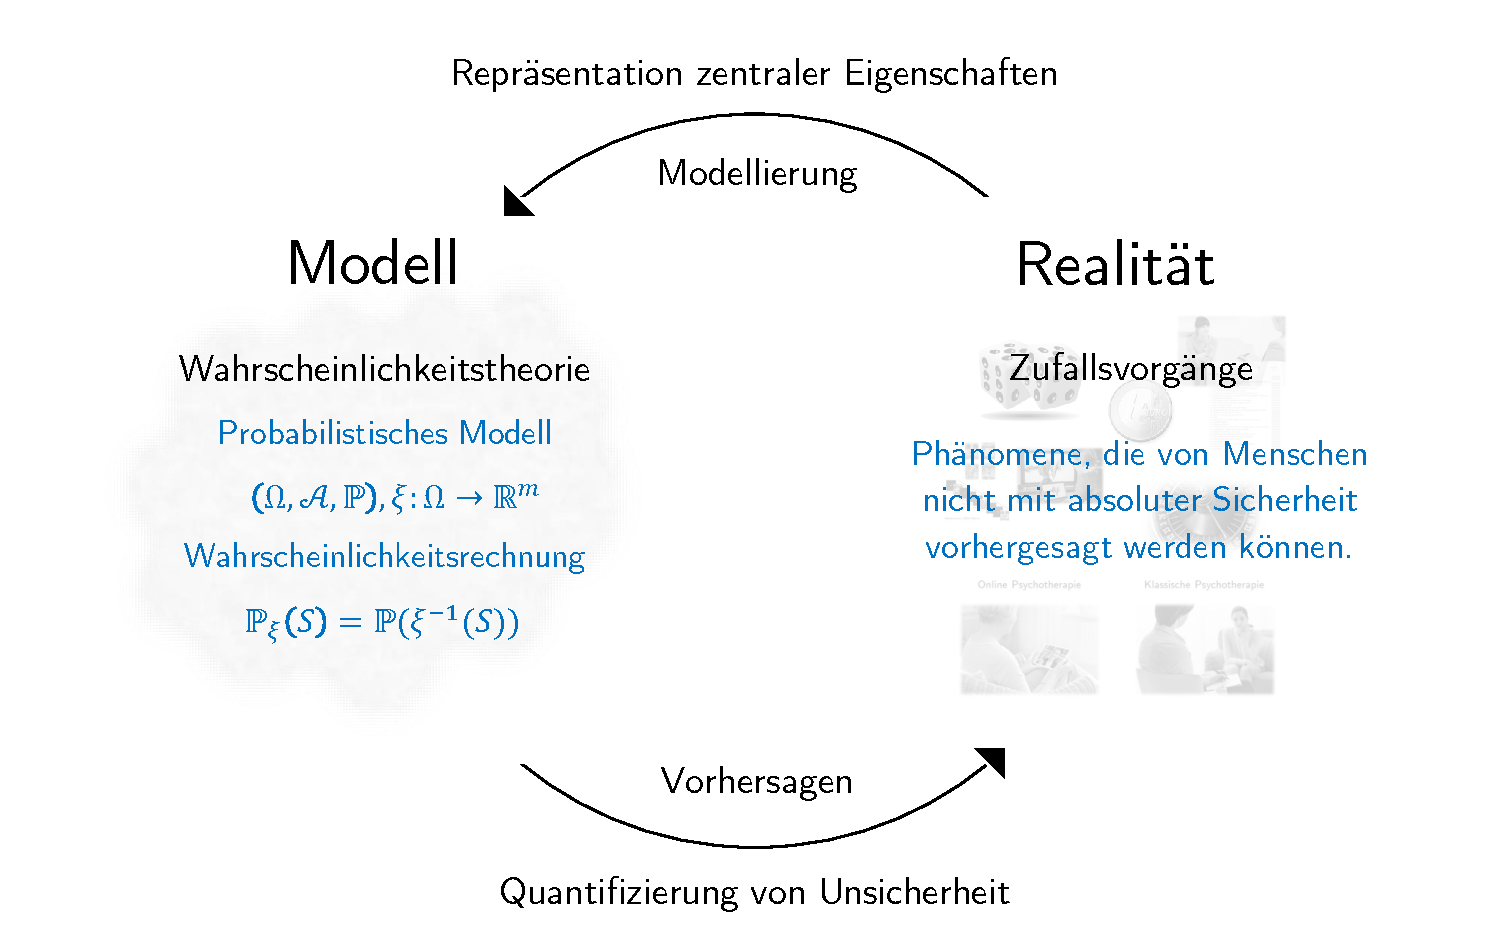
\includegraphics[width=0.9\linewidth]{5_Abbildungen/mvda_5_wahrscheinlichkeitstheorie_modell} \end{center}

\small
\center

\href{https://bit.ly/3SNh3nR}{\textcolor{darkblue}{BSc Psychologie | Grundlagen der Mathematik und Informatik}}

\href{https://bit.ly/3yT42Sj}{\textcolor{darkblue}{BSc Psychologie | Wahrscheinlichkeitstheorie und Frequentistische Inferenz}}
\end{frame}

\begin{frame}[fragile]{Vorbemerkungen}
\protect\hypertarget{vorbemerkungen-2}{}
\textcolor{darkblue}{Realisierungen von Zufallsvariablen} \footnotesize
\setstretch{1.1} \vspace{2mm}

\begin{Shaded}
\begin{Highlighting}[]
\CommentTok{\# Univariate Normalverteilungsparameter}
\NormalTok{mu      }\OtherTok{=} \FloatTok{2.0}                        \CommentTok{\# Erwartungswertparameter}
\NormalTok{sigsqr  }\OtherTok{=} \FloatTok{0.5}                        \CommentTok{\# Varianzparameter}
\NormalTok{n       }\OtherTok{=} \DecValTok{10}                         \CommentTok{\# Anzahl von u.i.v. Realisierungen}

\CommentTok{\# 10 Realisierungen}
\NormalTok{X       }\OtherTok{=} \FunctionTok{rnorm}\NormalTok{(n,mu,}\FunctionTok{sqrt}\NormalTok{(sigsqr))   }\CommentTok{\# \textbackslash{}xi\_i \textbackslash{}sim N(\textbackslash{}mu,\textbackslash{}sigma\^{}2), i = 1,...,n}
\FunctionTok{print}\NormalTok{(X)}
\end{Highlighting}
\end{Shaded}

\begin{verbatim}
>  [1] 1.010 2.181 0.277 1.996 2.440 2.812 0.712 1.825 1.827 1.800
\end{verbatim}

\begin{Shaded}
\begin{Highlighting}[]
\CommentTok{\# 10 Realisierungen}
\NormalTok{X       }\OtherTok{=} \FunctionTok{rnorm}\NormalTok{(n,mu,}\FunctionTok{sqrt}\NormalTok{(sigsqr))   }\CommentTok{\# \textbackslash{}xi\_i \textbackslash{}sim N(\textbackslash{}mu,\textbackslash{}sigma\^{}2), i = 1,...,n}
\FunctionTok{print}\NormalTok{(X)}
\end{Highlighting}
\end{Shaded}

\begin{verbatim}
>  [1] 1.608 2.445 3.460 0.847 2.362 0.683 1.631 1.963 2.384 1.354
\end{verbatim}
\end{frame}

\begin{frame}{Vorbemerkungen}
\protect\hypertarget{vorbemerkungen-3}{}
\textcolor{darkblue}{Wahrscheinlichkeitstheorie, Daten, Deskriptive Statistik}

\begin{center}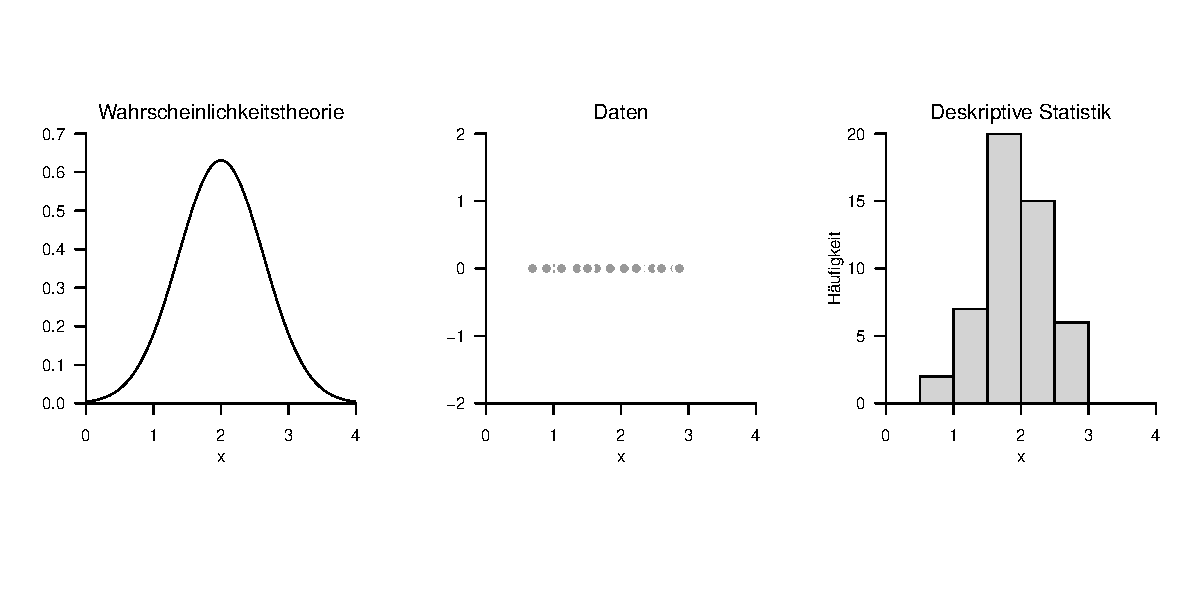
\includegraphics[width=1\linewidth]{5_Abbildungen/mvda_5_univariate_statistik} \end{center}
\end{frame}

\begin{frame}[fragile]{Vorbemerkungen}
\protect\hypertarget{vorbemerkungen-4}{}
\textcolor{darkblue}{Realisierungen von Zufallsvektoren} \footnotesize
\setstretch{1} \vspace{1mm}

\begin{Shaded}
\begin{Highlighting}[]
\CommentTok{\# R Paket für multivariate Normalverteilungsrealisierung}
\FunctionTok{library}\NormalTok{(MASS)}

\CommentTok{\# Multivariate Normalverteilungsparameter}
\NormalTok{mu      }\OtherTok{=} \FunctionTok{c}\NormalTok{(}\FloatTok{2.0}\NormalTok{,}\FloatTok{5.0}\NormalTok{)                 }\CommentTok{\# Erwartungswertparameter}
\NormalTok{Sigma   }\OtherTok{=} \FunctionTok{matrix}\NormalTok{(}\FunctionTok{c}\NormalTok{(}\FloatTok{0.5}\NormalTok{,}\FloatTok{0.1}\NormalTok{,          }\CommentTok{\# Kovarianzmatrixparamter}
                   \FloatTok{0.1}\NormalTok{,}\FloatTok{0.5}\NormalTok{),}
                 \AttributeTok{nrow =} \DecValTok{2}\NormalTok{,}
                 \AttributeTok{byrow =} \ConstantTok{TRUE}\NormalTok{)}
\NormalTok{n       }\OtherTok{=} \DecValTok{10}                         \CommentTok{\# Anzahl von u.i.v. Realisierungen}

\CommentTok{\# 10 Realisierungen}
\NormalTok{X       }\OtherTok{=} \FunctionTok{t}\NormalTok{(}\FunctionTok{mvrnorm}\NormalTok{(n,mu,Sigma))     }\CommentTok{\# \textbackslash{}xi\_i \textbackslash{}sim N(\textbackslash{}mu,\textbackslash{}Sigma), i = 1,...,n}
\FunctionTok{print}\NormalTok{(X)}
\end{Highlighting}
\end{Shaded}

\begin{verbatim}
>      [,1] [,2] [,3] [,4] [,5] [,6] [,7] [,8] [,9] [,10]
> [1,] 1.84 2.12 1.18 1.68 2.98 2.01 2.34 2.12 1.69 0.694
> [2,] 5.67 5.28 4.39 6.13 6.08 4.89 3.63 4.87 4.41 4.649
\end{verbatim}

\begin{Shaded}
\begin{Highlighting}[]
\CommentTok{\# 10 Realisierungen}
\NormalTok{X       }\OtherTok{=} \FunctionTok{t}\NormalTok{(}\FunctionTok{mvrnorm}\NormalTok{(n,mu,Sigma))     }\CommentTok{\# \textbackslash{}xi\_i \textbackslash{}sim N(\textbackslash{}mu,\textbackslash{}sigma\^{}2), i = 1,...,n}
\FunctionTok{print}\NormalTok{(X)}
\end{Highlighting}
\end{Shaded}

\begin{verbatim}
>      [,1] [,2] [,3] [,4] [,5] [,6] [,7] [,8] [,9] [,10]
> [1,] 1.65 1.76 2.06 1.85 2.23 3.26 3.04 1.12 2.23 0.857
> [2,] 5.42 4.54 4.88 4.87 5.26 6.76 4.01 6.52 4.90 4.048
\end{verbatim}
\end{frame}

\begin{frame}{Vorbemerkungen}
\protect\hypertarget{vorbemerkungen-5}{}
\small

\textcolor{darkblue}{Multivariate Wahrscheinlichkeitstheorie, Multivariate Daten, Multivariate Deskriptive Statistik}

\begin{center}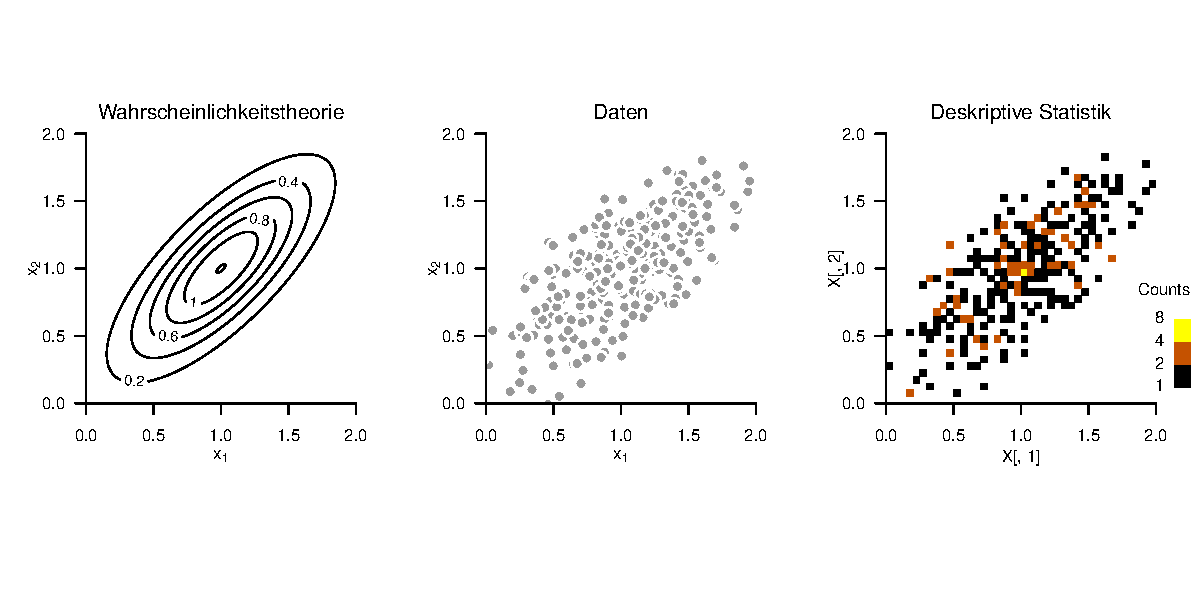
\includegraphics[width=1\linewidth]{5_Abbildungen/mvda_5_multivariate_statistik} \end{center}
\end{frame}

\begin{frame}{}
\protect\hypertarget{section-4}{}
\large
\setstretch{2.5}
\vfill

Vorbemerkungen

\textbf{Multivariate Verteilungen}

Marginalverteilungen und Bedingte Verteilungen

Erwartungswert, Kovarianzmatrizen und Korrelationsmatrizen

Selbstkontrollfragen \vfill
\end{frame}

\begin{frame}{Multivariate Verteilungen}
\protect\hypertarget{multivariate-verteilungen}{}
\footnotesize
\begin{definition}[Wahrscheinlichkeitsraum]
\justifying
Ein \textit{Wahrscheinlichkeitsraum} ist ein Triple $(\Omega, \mathcal{A}, \mathbb{P})$, wobei
\begin{itemize}
\item $\Omega$ eine beliebige nichtleere Menge von \textit{Ergebnissen} $\omega$ ist und \textit{Ergebnismenge} heißt,
\item $\mathcal{A}$ eine \textit{$\sigma$-Algebra auf $\Omega$} ist und \textit{Ereignissystem} heißt,
\item $\mathbb{P}$ eine Abbildung der Form $\mathbb{P}:\mathcal{A} \to [0,1]$ mit den Eigenschaften

\begin{itemize}

\begin{footnotesize}
\item[o] \textit{Nicht-Negativität} $\mathbb{P}(A) \ge 0$ für alle $A \in \mathcal{A}$,
\item[o] \textit{Normiertheit} $\mathbb{P}(\Omega) = 1$ und
\item[o] \textit{ $\sigma$-Additivität} $\mathbb{P}(\cup_{i=1}^\infty A_i) = \sum\limits_{i=1}^\infty \mathbb{P}(A_i)$
          für paarweise disjunkte $A_i \in \mathcal{A}$
\end{footnotesize}
\end{itemize}
ist und \textit{Wahrscheinlichkeitsmaß} heißt.
\end{itemize}
Das Tuple $(\Omega, \mathcal{A})$ aus Ergebnismenge und Ereignissystem wird
als \textit{Messraum} bezeichnet.
\end{definition}

Die stillschweigende Mechanik des Wahrscheinlichkeitsraummodells

\begin{itemize}
\tightlist
\item
  Wir stellen uns sequentielle \emph{Durchgänge} eines
  \emph{Zufallsvorgangs} vor.
\item
  In jedem Durchgang wird genau ein \(\omega\) aus \(\Omega\) mit
  Wahrscheinlichkeit \(\mathbb{P}(\{\omega\})\) \emph{realisiert}.
\item
  \(\mathbb{P}(\{\omega\})\) bestimmt, mit welcher Wahrscheinlichkeit
  \(\omega\) in einem Durchgang aus \(\Omega\) realisiert wird.
\item
  Wenn \(\omega \in A\) für \(A \in \mathcal{A}\) sagt man, dass das
  Ereignis \(A\) eingetreten ist.
\item
  Z.B. gilt beim Würfel für \(\omega = 2\) mit \(\omega \in \{2,4,6\}\),
  dass das Ereignis ``Eine gerade Zahl fällt'' eingetreten ist.
\end{itemize}
\end{frame}

\begin{frame}{Multivariate Verteilungen}
\protect\hypertarget{multivariate-verteilungen-1}{}
\footnotesize
\begin{definition}[Zufallsvektor]
\justifying
$(\Omega, \mathcal{A}, \mathbb{P})$ sei ein Wahrscheinlichkeitsraum und
$(\mathcal{X},\mathcal{S})$ sei ein $m$-dimensionaler Messraum.
Ein $m$-dimensionaler \textit{Zufallsvektor} ist definiert als eine Abbildung
\begin{equation}
\xi:\Omega \to \mathcal{X}, \omega \mapsto \xi(\omega) :=
\begin{pmatrix}
\xi_1(\omega) \\
\vdots      \\
\xi_m(\omega)
\end{pmatrix}
\end{equation}
mit der \textit{Messbarkeitseigenschaft}
\begin{equation}
\{\omega \in \Omega|\xi(\omega) \in S \} \in \mathcal{A} \mbox{ für alle } S \in \mathcal{S}.
\end{equation}
\end{definition}
\vspace{-2mm}
\footnotesize

Bemerkungen \vspace{-2mm}

\begin{itemize}
\tightlist
\item
  \(\xi\) ist hier eine univariate, vektorwertige Abbildung.
\item
  Das Standardbeispiel für \((\mathcal{X},\mathcal{S})\) ist
  \((\mathbb{R}^m, \mathcal{B}(\mathbb{R}^m))\).
\item
  Wir verzichten auf eine explizite Einführung \(m\)-dimensionaler
  \(\sigma\)-Algebren wie \(\mathcal{B}(\mathbb{R}^m)\).
\item
  Ohne Beweis halten wir fest, dass \(\xi\) messbar ist, wenn die
  Funktionen \(\xi_1,...,\xi_m\) messbar sind.
\item
  Die Komponentenfunktionen eines Zufallsvektors sind Zufallsvariablen.
\item
  Ein \(m\)-dimensionaler Zufallsvektor ist die Konkatenation von \(m\)
  Zufallsvariablen.
\item
  Für \(m := 1\) ist ein Zufallsvektor eine Zufallsvariable.
\item
  Für einen Zufallsvektor schreiben wir auch häufig
  \(\xi:= (\xi_1,...,\xi_m)\).
\end{itemize}
\end{frame}

\begin{frame}{Multivariate Verteilungen}
\protect\hypertarget{multivariate-verteilungen-2}{}
\vfill

\begin{center}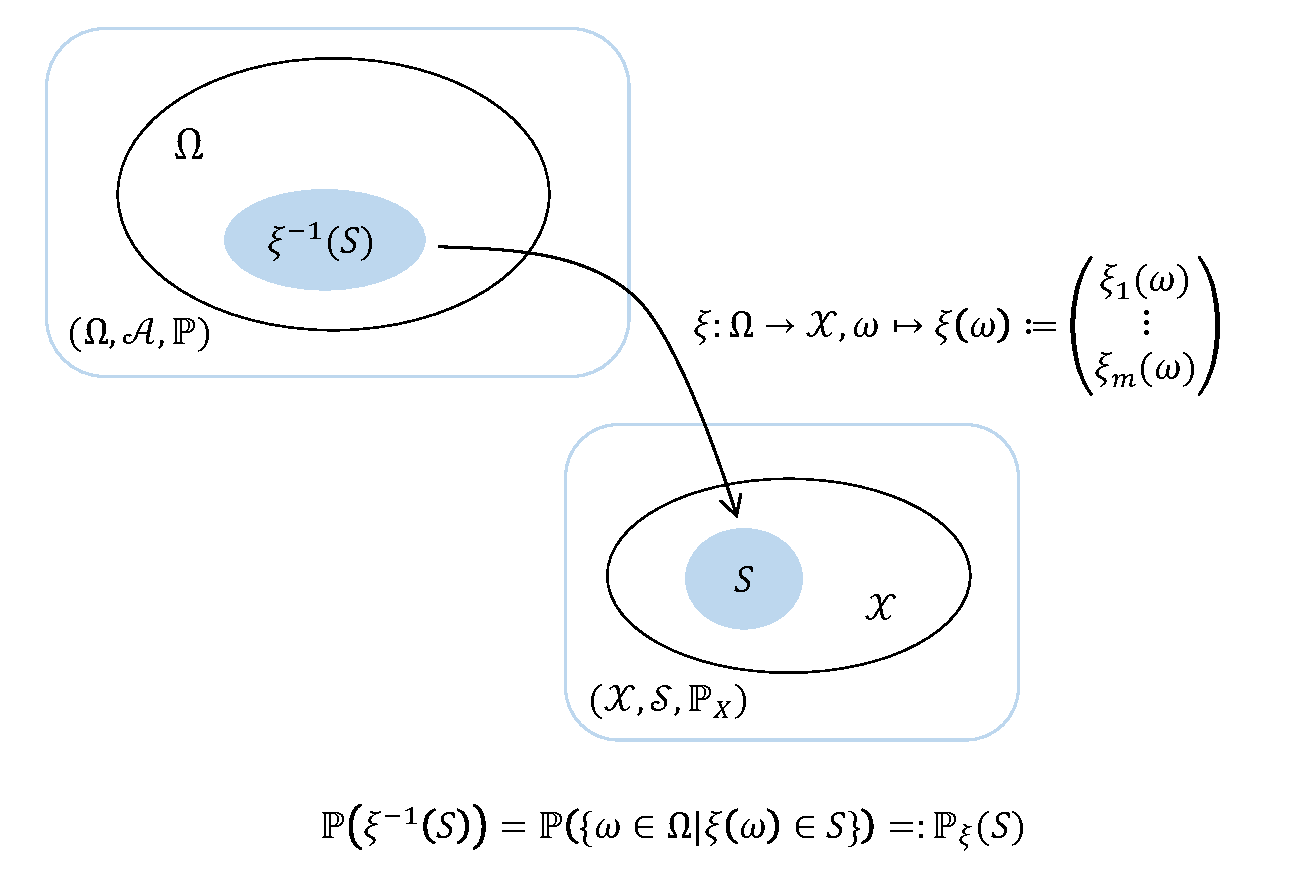
\includegraphics[width=0.9\linewidth]{5_Abbildungen/mvda_5_zufallsvektor} \end{center}
\vfill
\end{frame}

\begin{frame}{Multivariate Verteilungen}
\protect\hypertarget{multivariate-verteilungen-3}{}
\footnotesize
\begin{definition}[Multivariate Verteilung]
\justifying
$(\Omega, \mathcal{A}, \mathbb{P})$ sei ein Wahrscheinlichkeitsraum,
$(\mathcal{X},\mathcal{S})$ sei ein $m$-dimensionaler Messraum und
\begin{equation}
\xi : \Omega \to \mathcal{X}, \omega \mapsto \xi(\omega)
\end{equation}
sei ein Zufallsvektor. Dann heißt das Wahrscheinlichkeitsmaß $\mathbb{P}_\xi$,
definiert durch
\begin{equation}
\mathbb{P}_\xi : \mathcal{S} \to [0,1], S \mapsto \mathbb{P}_\xi(S)
:= \mathbb{P}(\xi^{-1}(S))
 = \mathbb{P}\left(\{\omega \in \Omega|\xi(\omega) \in S\}\right)
\end{equation}
die \textit{multivariate Verteilung des Zufallsvektor $\xi$}.
\end{definition}
\footnotesize

Bemerkungen

\begin{itemize}
\tightlist
\item
  Der Einfachheit halber spricht man oft auch nur von ``der Verteilung
  des Zufallsvektors \(\xi\)''.
\item
  Die Notationskonventionen für Zufallsvariablen gelten für
  Zufallsvektoren analog, z.B. \begin{align}
  \begin{split}
  \mathbb{P}_\xi(\xi \in S)
  & := \mathbb{P}\left(\{\xi \in S\} \right)
  = \mathbb{P}\left(\{\omega \in \Omega|\xi(\omega) \in S\} \right)
  \\
  \mathbb{P}_\xi(\xi = x)
  & := \mathbb{P}\left(\{\xi = x\} \right)
  = \mathbb{P}\left(\{\omega \in \Omega|\xi(\omega) = x\} \right)
  \\
  \mathbb{P}_\xi(\xi \le x)
  & := \mathbb{P}\left(\{\xi \le x\} \right)
  = \mathbb{P}\left(\{\omega \in \Omega|\xi(\omega) \le x\} \right)
  \\
  \mathbb{P}_\xi(x_1 \le \xi \le x_2)
  & := \mathbb{P}\left(\{x_1 \le \xi \le x_2\} \right)
   = \mathbb{P}\left(\{\omega \in \Omega|x_1 \le \xi(\omega) \le x_2\} \right)
  \end{split}
  \end{align}
\item
  Relationsoperatoren wie \(\le\) werden hier \textit{komponentenweise}
  verstanden.
\item
  Zum Beispiel heißt \(x \le y\) für \(x,y \in \mathbb{R}^m\), dass
  \(x_i \le y_i\) für alle \(i = 1,...,m\).
\end{itemize}
\end{frame}

\begin{frame}{Multivariate Verteilungen}
\protect\hypertarget{multivariate-verteilungen-4}{}
\small
\begin{definition}[Multivariate kumulative Verteilungsfunktionen]
$\xi$ sei ein Zufallsvektor mit Ergebnisraum $\mathcal{X}$. Dann heißt eine Funktion
der Form
\begin{equation}
P_\xi : \mathcal{X} \to [0,1],\, x \mapsto P_\xi(x) := \mathbb{P}_\xi(\xi \le x)
\end{equation}
multivariate kumulative Verteilungsfunktion von $\xi$.
\end{definition}

Bemerkung

\begin{itemize}
\tightlist
\item
  \justifying Multivariate kumulative Verteilungsfunktionen können zur
  Definition von multivariaten Verteilungen genutzt werden, häufiger ist
  allerdings die Definition multivariater Verteilungen durch
  multivariate Wahrscheinlichkeitsmasse- oder
  Wahrscheinlichkeitsdichtefunktionen.
\end{itemize}
\end{frame}

\begin{frame}{Multivariate Verteilungen}
\protect\hypertarget{multivariate-verteilungen-5}{}
\small
\begin{definition}[Diskreter Zufallsvektor, Multivariate WMF]
\justifying
$\xi$ sei ein Zufallsvektor mit Ergebnisraum $\mathcal{X}$. $\xi$ heißt
\textit{diskreter Zufallsvektor} wenn der Ergebnisraum $\mathcal{X}$ endlich oder
abzählbar ist und eine Funktion der Form
\begin{equation}
p_\xi : \mathcal{X} \to [0,1], x \mapsto p_\xi(x)
\end{equation}
existiert, für die gilt
\begin{itemize}
\item[(1)] $\sum_{x \in \mathcal{X}}p_\xi(x) = 1$ und
\item[(2)] $\mathbb{P}_\xi(\xi = x) = p_\xi(x)$ für alle $x \in \mathcal{X}$.
\end{itemize}
Ein entsprechende Funktion $p$ heißt \textit{multivariate Wahrscheinlichkeitsmassefunktion (WMF)} von $\xi$.
\end{definition}

Bemerkungen

\begin{itemize}
\tightlist
\item
  Der Begriff der multivariaten WMF ist analog zum Begriff der WMF.
\item
  Man spricht oft einfach von der WMF eines Zufallsvektors.
\item
  Wie univariate WMFen sind multivariate WMFen nicht-negativ und
  normiert.
\end{itemize}
\end{frame}

\begin{frame}{Multivariate Verteilungen}
\protect\hypertarget{multivariate-verteilungen-6}{}
Beispiel (Multivariate Wahrscheinlichkeitsmassefunktion)

\vspace{2mm}

\small
\justifying

Wir betrachten einen zweidimensionalen Zufallsvektor
\(\xi:= (\xi_1,\xi_2)\) der Werte in
\(\mathcal{X} := \mathcal{X}_1 \times \mathcal{X}_2\) annimmt, wobei
\(\mathcal{X}_1 := \{1,2,3\}\) und \(\mathcal{X}_2 = \{1,2,3,4\}\)
seien.

Eine exemplarische bivariate WMF der Form \begin{equation}
p_\xi: \{1,2,3\} \times \{1,2,3,4\} \to [0,1], (x_1,x_2) \mapsto p_\xi(x_1,x_2)
\end{equation} ist dann durch nachfolgende Tabelle definiert:
\vspace{1mm}

\begin{table}\label{tab:wmf_bivariat}
\begin{center}
\begin{tabular}{|c|cccc|}
\hline
$p_\xi(x_1,x_2)$    &   $x_2 = 1$   &   $x_2 = 2$   &   $x_2 = 3$   &   $x_2 = 4$   \\\hline
$x_1 = 1$       &   $0.1$       &   $0.0$       &   $0.2$       &   $0.1$       \\
$x_1 = 2$       &   $0.1$       &   $0.2$       &   $0.0$       &   $0.0$       \\
$x_1 = 3$       &   $0.0$       &   $0.1$       &   $0.1$       &   $0.1$       \\\hline
\end{tabular}
\end{center}
\end{table}
\vspace{1mm}

Man beachte, dass
\(\sum_{x \in \mathcal{X}} p_\xi(x) = \sum_{x_1 = 1}^3 \sum_{x_2 = 1}^4 p_\xi(x_1,x_2) = 1\).
\end{frame}

\begin{frame}{Multivariate Verteilungen}
\protect\hypertarget{multivariate-verteilungen-7}{}
\small
\begin{definition}[Kontinuierlicher Zufallsvektor, Multivariate WDF]
\justifying
Ein Zufallsvektor $\xi$ heißt \textit{kontinuierlich}, wenn $\mathbb{R}^m$ der
Ergebnisraum von $\xi$ ist und eine Funktion
\begin{equation}
p_\xi : \mathbb{R}^m \to \mathbb{R}_{\ge 0}, x \mapsto p_\xi(x),
\end{equation}
existiert, für die gilt
\begin{itemize}
\item[(1)] $\int_{\mathbb{R}^m} p_\xi(x)\,dx = 1$ und
\item[(2)] $\mathbb{P}_\xi(x_1 \le \xi \le x_2)
            = \int_{x_{1_1}}^{x_{2_1}} \cdots \int_{x_{1_m}}^{x_{2_m}} p_\xi(s_1,...,s_m)\,ds_1 \cdots ds_m$.
\end{itemize}
Eine entsprechende Funktion $p$ heißt \textit{multivariate Wahrscheinlichkeitsdichtefunktion (WDF)} von $\xi$.
\end{definition}

\footnotesize

Bemerkungen

\begin{itemize}
\tightlist
\item
  Der Begriff der multivariaten WDF ist analog zum Begriff der WDF.
\item
  Man spricht häufig auch einfach von der WDF eines Zufallsvektors
\item
  Wie univariate WDFen sind multivariate WDFen nicht-negativ und
  normiert.
\item
  Wie für kontinuierliche Zufallsvariablen gilt für kontinuierliche
  Zufallsvektoren \begin{equation}
  \mathbb{P}_\xi(\xi = x)
  = \mathbb{P}_\xi(x \le \xi \le x)
  = \smallint_{x_1}^{x_1} \cdots \smallint_{x_m}^{x_m} p_\xi(s_1,...,s_m)\,ds_1 \cdots ds_m
  = 0
  \end{equation}
\item
  In (6) Multivariate Normalverteilungen befassen wir uns mit dem
  Standardbeispiel für multivariate WDFen.
\end{itemize}
\end{frame}

\begin{frame}{}
\protect\hypertarget{section-5}{}
\large
\setstretch{2.5}
\vfill

Vorbemerkungen

Multivariate Verteilungen

\textbf{Marginalverteilungen und Bedingte Verteilungen}

Erwartungswert, Kovarianzmatrizen und Korrelationsmatrizen

Selbstkontrollfragen \vfill
\end{frame}

\begin{frame}{Marginalverteilungen und Bedingte Verteilungen}
\protect\hypertarget{marginalverteilungen-und-bedingte-verteilungen}{}
\small
\begin{definition}[Univariate Marginalverteilung]
\justifying
$(\Omega, \mathcal{A}, \mathbb{P})$ sei ein Wahrscheinlichkeitsraum,
$(\mathcal{X}, \mathcal{S})$ sei ein $m$-dimensionaler Messraum,
$\xi:\Omega \to \mathcal{X}$ sei ein Zufallsvektor, $\mathbb{P}_\xi$ sei die
Verteilung von $\xi$, $\mathcal{X}_i \subset \mathcal{X}$ sei der Ergebnisraum der
$i$ten Komponente $\xi_i$ von $\xi$, und $\mathcal{S}_i$ sei eine
$\sigma$-Algebra auf $\xi_i$. Dann heißt die durch
\begin{equation}
\mathbb{P}_{\xi_i} : \mathcal{S}_i \to [0,1],
S \mapsto  \mathbb{P}_\xi\left(\mathcal{X}_1
                     \times
                     \cdots
                     \times
                     \mathcal{X}_{i-1}
                     \times S
                     \times \mathcal{X}_{i+1}
                     \times \cdots
                     \times \mathcal{X}_m\right)
\mbox{ für } S \in \mathcal{S}_i
\end{equation}
definierte Verteilung die \textit{$i$te univariate Marginalverteilung von $\xi$}.
\end{definition}

Bemerkungen

\begin{itemize}
\tightlist
\item
  \justifying Univariate Marginalverteilungen sind die Verteilungen der
  Komponenten eines Zufallsvektors.
\item
  Univariate Marginalverteilungen sind Verteilungen von
  Zufallsvariablen.
\item
  Die Festlegung der multivariaten Verteilung von \(\xi\) legt auch die
  Verteilungen der \(\xi_i\) fest.
\end{itemize}
\end{frame}

\begin{frame}{Marginalverteilungen und Bedingte Verteilungen}
\protect\hypertarget{marginalverteilungen-und-bedingte-verteilungen-1}{}
\footnotesize
\begin{theorem}[Marginale Wahrscheinlichkeitsmasse- und dichtefunktionen]
\justifying
\normalfont
(1) $\xi= (\xi_1,...,\xi_m)$ sei ein $m$-dimensionaler diskreter Zufallsvektor
mit Wahrscheinlichkeitsmassefunktion $p_\xi$ und Komponentenergebnisräumen
$\mathcal{X}_1, ..., \mathcal{X}_m$. Dann ergibt sich die
Wahrscheinlichkeitsmassefunktion der $i$ten Komponente $\xi_i$ von $\xi$ als
\begin{multline}
p_{\xi_i} : \mathcal{X}_i \to [0,1], x_i \mapsto p_{\xi_i}(x_i) := \\
\sum_{x_1} \cdots \sum_{x_{i-1}} \sum_{x_{i+1}} \cdots \sum_{x_m} p_\xi(x_1,...,x_{i-1},x_i,x_{i+1}, ...,x_m).
\end{multline}
(2) $\xi= (\xi_1,...,\xi_m)$ sei ein $m$-dimensionaler kontinuierlicher Zufallsvektor
mit Wahrscheinlichkeitsdichtefunktion $p_\xi$ und Komponentenergebnisraum $\mathbb{R}$.
Dann ergibt sich die Wahrscheinlichkeitsdichtefunktion der $i$ten Komponente $\xi_i$ von $\xi$ als
\begin{multline}
p_{\xi_i} : \mathbb{R} \to \mathbb{R}_{\ge 0},  x_i \mapsto p_{\xi_i}(x_i) :=  \\
\smallint_{x_1} \cdots \smallint_{x_{i-1}} \smallint_{x_{i+1}} \cdots \smallint_{x_m}
   p_\xi(x_1,..., x_{i-1},x_i,x_{i+1}, ...,x_m)
   \,dx_1...\,dx_{i-1}\,dx_{i+1}...\,dx_m.
\end{multline}
\end{theorem}
\vspace{-2mm}

Bemerkungen \vspace{-1mm}

\begin{itemize}
\tightlist
\item
  \justifying Wir verzichten auf einen Beweis.
\item
  Die WMFen der univariaten Marginalverteilungen diskreter
  Zufallsvektoren ergeben sich durch Summation.
\item
  Die WDFen der univariaten Marginalverteilungen kontinuierlicher
  Zufallsvektoren ergeben sich durch Integration.
\end{itemize}
\end{frame}

\begin{frame}{Marginalverteilungen und Bedingte Verteilungen}
\protect\hypertarget{marginalverteilungen-und-bedingte-verteilungen-2}{}
Beispiel (Marginale Wahrscheinlichkeitsmassefunktionen)

\vspace{2mm}

\small
\justifying

Wir betrachten erneut den zweidimensionalen Zufallsvektor
\(\xi:= (\xi_1,\xi_2)\) der Werte in
\(\mathcal{X} := \mathcal{X}_1 \times \mathcal{X}_2\) annimmt, wobei
\(\mathcal{X}_1 := \{1,2,3\}\) und \(\mathcal{X}_2 = \{1,2,3,4\}\)
seien. \vspace{1mm}

Basierend auf der oben definierten WMF ergeben sich folgende marginale
WMFen \(p_{\xi_1}\) und \(p_{\xi_2}\): \vspace{2mm}

\begin{table}\label{tab:wmf_marginal}
\begin{center}
\begin{tabular}{|c|cccc|c|}
\hline
$p_\xi(x_1,x_2)$    &   $x_2 = 1$   &   $x_2 = 2$   &   $x_2 = 3$   &   $x_2 = 4$   & $p_{\xi_1}(x_1)$  \\\hline
$x_1 = 1$           &   $0.1$       &   $0.0$       &   $0.2$       &   $0.1$       & $0.4$             \\
$x_1 = 2$           &   $0.1$       &   $0.2$       &   $0.0$       &   $0.0$       & $0.3$             \\
$x_1 = 3$           &   $0.0$       &   $0.1$       &   $0.1$       &   $0.1$       & $0.3$             \\\hline
$p_{\xi_2}(x_2)$    &   $0.2$       &   $0.3$       &   $0.3$       &   $0.2$       &                   \\\hline
\end{tabular}
\end{center}
\end{table}
\vspace{2mm}

Man beachte, dass \(\sum_{x_1 = 1}^3 p_{\xi_1}(x_1) = 1\) und
\(\sum_{x_2 = 1}^3 p_{\xi_2}(x_2) = 1\) gilt.
\end{frame}

\begin{frame}{Marginalverteilungen und Bedingte Verteilungen}
\protect\hypertarget{marginalverteilungen-und-bedingte-verteilungen-3}{}
\small

Vorbemerkungen zu Bedingten Verteilungen

\footnotesize

Wir erinnern uns, dass für einen Wahrscheinlichkeitsraum
\((\Omega, \mathcal{A}, \mathbb{P})\) und zwei Ereignisse
\(A,B \in \mathcal{A}\) mit \(\mathbb{P}(B) > 0\) die bedingte
Wahrscheinlichkeit von \(A\) gegeben \(B\) definiert ist als
\begin{equation}
\mathbb{P}(A|B) = \frac{\mathbb{P}(A \cap B)}{\mathbb{P}(B)}.
\end{equation}

Analog wird für zwei Zufallsvariablen \(\xi_1,\xi_2\) mit Ereignisräumen
\(\mathcal{X}_1,\mathcal{X}_2\) und (messbaren) Mengen
\(S_1 \in \mathcal{X}_1, S_2 \in \mathcal{X}_2\) die bedingte Verteilung
von \(\xi_1\) gegeben \(\xi_2\) mithilfe der Ereignisse \begin{equation}
A := \{\xi_1 \in S_1\} \mbox{ und } B := \{\xi_2 \in S_2\}
\end{equation} definiert. \vspace{1mm}

So ergibt sich zum Beispiel die bedingte Wahrscheinlichkeit, dass
\(\xi_1 \in S_1\) gegeben dass \(\xi_2 \in S_2\) unter der Annahme, dass
\(\mathbb{P}(\{\xi_2 \in S_2\}) > 0\), zu \begin{equation}
\mathbb{P}( \{\xi_1 \in S_1\}|\{\xi_2 \in S_2\})
= \frac{\mathbb{P}(\{\xi_1 \in S_1\} \cap \{\xi_2 \in S_2\})}{\mathbb{P}(\{\xi_2 \in S_2\})}.
\end{equation}

Wir betrachten zunächst durch WMFen/WDFen zweidimensionaler
Zufallsvektoren definierte bedingte Verteilungen.
\end{frame}

\begin{frame}{Marginalverteilungen und Bedingte Verteilungen}
\protect\hypertarget{marginalverteilungen-und-bedingte-verteilungen-4}{}
\footnotesize
\begin{definition}[Bedingte WMF, diskrete bedingte Verteilung]
\justifying
$\xi:= (\xi_1,\xi_2)$ sei ein diskreter Zufallsvektor mit $m + k$ dimensionalen Ergebnisraum
$\mathcal{X} := \mathcal{X}_1 \times \mathcal{X}_2$, WMF $p_\xi = p_{\xi_1,\xi_2}$
und marginalen WMFen $p_{\xi_1}$ und $p_{\xi_2}$. Die bedingte WMF von $\xi_1$ gegeben
$\xi_2 = x_2$ ist dann für $p_{\xi_2}(x_2) > 0$ definiert als
\begin{equation}
p_{\xi_1|\xi_2 = x_2} : \mathcal{X}_1 \to [0,1],
x_1 \mapsto p_{\xi_1|\xi_2 = x_2}(x_1|x_2) := \frac{p_{\xi_1,\xi_2}(x_1,x_2)}{p_{\xi_2}(x_2)}
\end{equation}
Analog ist für $p_{\xi_1}(x_1) > 0$ die bedingte WMF von $\xi_2$ gegeben $\xi_1 = x_1$
definiert als
\begin{equation}
p_{\xi_2|\xi_1 = x_1} : \mathcal{X}_2 \to [0,1],
x_2 \mapsto p_{\xi_2|\xi_1 = x_2}(x_1|x_2) := \frac{p_{\xi_1,\xi_2}(x_1,x_2)}{p_{\xi_1}(x_1)}
\end{equation}
Die bedingten Verteilungen mit WMFen $p_{\xi_1|\xi_2 = x_2}$ und $p_{\xi_2|\xi_1 = x_1}$
heißen dann die \textit{diskreten bedingten Verteilungen von $\xi_1$ gegeben $\xi_2 = x_2$
und $\xi_2$ gegeben $\xi_1 = x_1$}, respektive.
\end{definition}

Bemerkungen

\begin{itemize}
\tightlist
\item
  In Analogie zur Definition der bedingten Wahrscheinlichkeit von
  Ereignissen gilt also \begin{equation}
  p_{\xi_1|\xi_2}(x_1|x_2)
  = \frac{p_{\xi_1,\xi_2}(x_1,x_2)}{p_{\xi_2}(x_2)}
  = \frac{\mathbb{P}(\{\xi_1 = x_1\} \cap \{\xi_2 = x_2\})}{\mathbb{P}(\{\xi_2 = x_2\})}.
  \end{equation}
\item
  Bedingte Verteilungen sind (lediglich) normalisierte gemeinsame
  Verteilungen.
\end{itemize}
\end{frame}

\begin{frame}{Marginalverteilungen und Bedingte Verteilungen}
\protect\hypertarget{marginalverteilungen-und-bedingte-verteilungen-5}{}
Beispiel (Bedingte Wahrscheinlichkeitsmassefunktionen)

\vspace{2mm}

\small
\justifying

Wir betrachten erneut den zweidimensionalen Zufallsvektor
\(\xi:= (\xi_1,\xi_2)\) der Werte in
\(\mathcal{X} := \mathcal{X}_1 \times \mathcal{X}_2\) annimmt, wobei
\(\mathcal{X}_1 := \{1,2,3\}\) und \(\mathcal{X}_2 = \{1,2,3,4\}\)
seien.

Basierend auf der oben definierten WMF und den entsprechenden oben
evaluierten marginalen WMFen ergeben sich folgende bedingte WMFen für
\(p_{\xi_2|\xi_1 = x_1}\) \vspace{1mm}

\renewcommand{\arraystretch}{1.4}
\begin{center}
\begin{tabular}{|c|cccc|}
\hline
$p_{\xi_2|\xi_1}(x_2|x_1)$
&   $x_2 = 1$
&   $x_2 = 2$
&   $x_2 = 3$
&   $x_2 = 4$
\\\hline
$p_{\xi_2|\xi_1 = 1}(x_2|x_1 = 1)$

&   $\frac{0.1}{0.4} = 0.25$

&   $\frac{0.0}{0.4} = 0.00$

&   $\frac{0.2}{0.4} = 0.50$

&   $\frac{0.1}{0.4} = 0.25$
\\
$p_{\xi_2|\xi_1 = 2}(x_2|x_1 = 2)$

&   $\frac{0.1}{0.3} = 0.3\bar{3}$

&   $\frac{0.2}{0.3} = 0.6\bar{6}$

&   $\frac{0.0}{0.3} = 0.00$

&   $\frac{0.0}{0.3} = 0.00$
\\
$p_{\xi_2|\xi_1 = 3}(x_2|x_1 = 3)$

&   $\frac{0.0}{0.3} = 0.00$

&   $\frac{0.1}{0.3} = 0.3\bar{3}$

&   $\frac{0.1}{0.3} = 0.3\bar{3}$

&   $\frac{0.1}{0.3} = 0.3\bar{3}$
\\\hline
\end{tabular}
\end{center}

\footnotesize

Bemerkungen

\begin{itemize}
\tightlist
\item
  Man beachte, dass
  \(\sum_{x_2 = 1}^4 p_{\xi_2|\xi_1 = x_1}(x_2|x_1) = 1\) für alle
  \(x_1 \in \mathcal{X}_1\).
\item
  Man beachte die qualitative Ähnlichkeit der WMFen
  \(p_{\xi_1,\xi_2}(x_1,x_2)\) und \(p_{\xi_2|\xi_1}(x_2|x_1)\).
\item
  Bedingte Verteilungen sind (lediglich) normalisierte gemeinsame
  Verteilungen.
\end{itemize}
\end{frame}

\begin{frame}{Marginalverteilungen und Bedingte Verteilungen}
\protect\hypertarget{marginalverteilungen-und-bedingte-verteilungen-6}{}
\footnotesize
\begin{definition}[Bedingte WDF, kontinuierliche bedingte Verteilungen]
\justifying
$\xi:= (\xi_1,\xi_2)$ sei ein kontinuierlicher Zufallsvektor mit Ergebnisraum
$\mathbb{R}^{m+k}$, WDF $p_\xi = p_{\xi_1,\xi_2}$ und marginalen WDFen $p_{\xi_1}$ und $p_{\xi_2}$.
Die bedingte WDF von $\xi_1$ gegeben $\xi_2 = x_2$ ist dann für $p_{\xi_2}(x_2) > 0$ definiert als
\begin{equation}
p_{\xi_1|\xi_2 = x_2} : \mathbb{R} \to \mathbb{R}_{\ge 0},
x_1 \mapsto p_{\xi_1|\xi_2 = x_2}(x_1|x_2) := \frac{p_{\xi_1,\xi_2}(x_1,x_2)}{p_{\xi_2}(x_2)}
\end{equation}
Analog ist für $p_{\xi_1}(x_1) > 0$ die bedingte WMF von $\xi_2$ gegeben $\xi_1 = x_1$ definiert als
\begin{equation}
p_{\xi_2|\xi_1 = x_1} : \mathbb{R} \to \mathbb{R}_{\ge 0},
x_2 \mapsto p_{\xi_2|\xi_1 = x_2}(x_2|x_1) := \frac{p_{\xi_1,\xi_2}(x_1,x_2)}{p_{\xi_1}(x_1)}
\end{equation}

Die Verteilungen mit WDFen $p_{\xi_1|\xi_2 = x_2}$ und $p_{\xi_2|\xi_1 = x_1}$ heißen dann
die \textit{kontinuierlichen bedingten Verteilungen von $\xi_1$ gegeben $\xi_2 = x_2$
und $\xi_2$ gegeben $\xi_1 = x_1$}, respektive.
\end{definition}

Bemerkung

\begin{itemize}
\tightlist
\item
  Im kontinuierlichen Fall gilt zwar \(\mathbb{P}_\xi(\xi = x) = 0\),
  aber nicht notwendig auch \(p_\xi(x) = 0\).
\item
  In Einheit (6) Multivariate Normalverteilung beschäftigen wir uns
  eingehend mit einem Beispiel.
\end{itemize}
\end{frame}

\begin{frame}{}
\protect\hypertarget{section-6}{}
\large
\setstretch{2.5}
\vfill

Vorbemerkungen

Multivariate Verteilungen

Marginalverteilungen und Bedingte Verteilungen

\textbf{Erwartungswert, Kovarianzmatrizen und Korrelationsmatrizen}

Selbstkontrollfragen \vfill
\end{frame}

\begin{frame}{Erwartungswert, Kovarianzmatrizen und
Korrelationsmatrizen}
\protect\hypertarget{erwartungswert-kovarianzmatrizen-und-korrelationsmatrizen}{}
\setstretch{1.2}
\footnotesize
\begin{definition}[Erwartungswert, Varianz, Kovarianz, Korrelation]
$\xi$ und $\ups$ seien Zufallsvariablen auf einem Wahrscheinlichkeitsraum $(\Omega, \mathcal{A}, \mathbb{P})$.
\begin{itemize}
\item Der \textit{Erwartungswert von $\xi$} definiert als
\begin{itemize}
\begin{footnotesize}
\item
$\mathbb{E}(\xi)
:=
\sum_{x \in \mathcal{X}} x\,p_\xi(x)$,
wenn $\xi: \Omega \to \mathcal{X}$ diskret mit WMF $p_\xi$ ist, und als
\item
$\mathbb{E}(\xi)
:=
\intinf x \,p_\xi(x)\,dx$,
wenn $\xi : \Omega \to \mathbb{R}$ kontinuierlich mit WDF $p_\xi$ ist.
\end{footnotesize}
\end{itemize}
\item Die \textit{Varianz von $\xi$} ist definiert als
\begin{equation}
\mathbb{V}(\xi) := \mathbb{E}\left((\xi - \mathbb{E}(\xi))^2\right).
\end{equation}
\item Die \textit{Kovarianz von $\xi$ und $\ups$} definiert als
\begin{equation}
\mathbb{C}(\xi,\ups) :=
\mathbb{E}\left(\left(\xi - \mathbb{E}(\xi) \right)\left(\ups - \mathbb{E}(\ups)\right)\right).
\end{equation}
\item Die \textit{Korrelation von $\xi$ und $\ups$} ist definiert als
\begin{equation}
\rho(\xi,\ups)
:= \frac{\mathbb{C}(\xi,\ups)}{\sqrt{\mathbb{V}(\xi)}\sqrt{\mathbb{V}(\ups)}}.
\end{equation}
\end{itemize}
\end{definition}
\vspace{-2mm}

Bemerkung \vspace{-2mm}

\begin{itemize}
\tightlist
\item
  Es gilt \(\mathbb{C}(\xi,\xi) = \mathbb{V}(\xi)\).
\item
  Für eine ausführliche Diskussion der Begriffe, siehe
  \href{https://bit.ly/3yT42Sj}{\textcolor{darkblue}{Wahrscheinlichkeitstheorie und Frequentistische Inferenz}}.
\item
  Die Begriffe sind nicht identisch mit den Begriffen des
  Stichprobenmittels und der Stichproben(ko)varianz.
\item
  Die Begriffe sind nicht identisch mit den Normalverteilungsparametern.
\end{itemize}
\end{frame}

\begin{frame}{Erwartungswert, Kovarianzmatrizen und
Korrelationsmatrizen}
\protect\hypertarget{erwartungswert-kovarianzmatrizen-und-korrelationsmatrizen-1}{}
\small
\begin{definition}[Erwartungswert eines Zufallsvektors]
\justifying
$\xi$ sei ein $m$-dimensionaler Zufallvektor. Dann ist der \textit{Erwartungwert}
von $\xi$ definiert als
\begin{equation}
\mathbb{E}(\xi) :=
\begin{pmatrix}
\mathbb{E}(\xi_1) \\
\vdots  \\
\mathbb{E}(\xi_m) \\
\end{pmatrix}.
\end{equation}
\end{definition}
\footnotesize

Bemerkungen

\begin{itemize}
\tightlist
\item
  Der Erwartungswert von \(\xi\) ist der Vektor der Erwartungswerte
  \(\mathbb{E}(\xi_1), ..., \mathbb{E}(\xi_m)\).
\item
  Im ALM \(y = X\beta + \varepsilon\) ist zum Beispiel
  \(\mathbb{E}(\varepsilon) = 0_n\) und
  \(\mathbb{E}(y) = X\beta \in \mathbb{R}^n\).
\end{itemize}
\end{frame}

\begin{frame}{Erwartungswert, Kovarianzmatrizen und
Korrelationsmatrizen}
\protect\hypertarget{erwartungswert-kovarianzmatrizen-und-korrelationsmatrizen-2}{}
\small
\begin{definition}[Kovarianzmatrix]
\justifying
$\xi$ sei ein $m$-dimensionaler Zufallsvektor. Dann ist die \textit{Kovarianzmatrix}
von $\xi$ definiert als
\begin{align}
\begin{split}
\mathbb{C}(\xi)
:= \mathbb{E}\left((\xi - \mathbb{E}(\xi))(\xi - \mathbb{E}(\xi))^T \right)
 =
\begin{pmatrix}
\mathbb{C}(\xi_1,\xi_1) & \cdots & \mathbb{C}(\xi_1,\xi_m) \\
\vdots              & \ddots & \vdots            \\
\mathbb{C}(\xi_m,\xi_1) & \cdots & \mathbb{C}(\xi_m,\xi_m) \\
\end{pmatrix}.
\end{split}
\end{align}
\end{definition}
\footnotesize

Bemerkungen

\begin{itemize}
\tightlist
\item
  Die Kovarianzmatrix \(\mathbb{C}(\xi)\) ist die \(m \times m\) Matrix
  der Kovarianzen \(\mathbb{C}(\xi_i,\xi_j), i,j = 1,...,m\).
\item
  Im ALM mit sphärischer Kovarianmatrix gilt per Definition
  \(\mathbb{C}(\varepsilon) = \mathbb{C}(y) = \sigma^2 I_n \in \mathbb{R}^{n \times n}\).
\item
  Die Äquivalenz der Kovarianzmatrixschreibweisen folgt wie im Folgenden
  dargestellt.
\end{itemize}
\end{frame}

\begin{frame}{Erwartungswert, Kovarianzmatrizen und
Korrelationsmatrizen}
\protect\hypertarget{erwartungswert-kovarianzmatrizen-und-korrelationsmatrizen-3}{}
\vspace{2mm}
\footnotesize
\setstretch{1}

Bemerkungen (fortgeführt) \begin{align}
\begin{split}
& \mathbb{E}\left((\xi - \mathbb{E}(\xi))(\xi - \mathbb{E}(\xi))^T \right) \\
& =
\mathbb{E}
\left(
\left(
\begin{pmatrix}
\xi_1 \\
\vdots \\
\xi_m
\end{pmatrix}
-
\begin{pmatrix}
\mathbb{E}(\xi_1) \\
\vdots \\
\mathbb{E}(\xi_m)
\end{pmatrix}
\right)
\left(
\begin{pmatrix}
\xi_1 \\
\vdots \\
\xi_m
\end{pmatrix}
-
\begin{pmatrix}
\mathbb{E}(\xi_1) \\
\vdots \\
\mathbb{E}(\xi_m)
\end{pmatrix}
\right)^T
\right)
\\
& =
\mathbb{E}
\left(
\begin{pmatrix}
\xi_1 - \mathbb{E}(\xi_1) \\
\vdots \\
\xi_m - \mathbb{E}(\xi_m)
\end{pmatrix}
\begin{pmatrix}
\xi_1 - \mathbb{E}(\xi_1)\\
\vdots \\
\xi_m - \mathbb{E}(\xi_m)
\end{pmatrix}^T
\right)
\\
& =
\mathbb{E}
\left(
\begin{pmatrix}
\xi_1 - \mathbb{E}(\xi_1) \\
\vdots \\
\xi_m - \mathbb{E}(\xi_m)
\end{pmatrix}
\begin{pmatrix}
\xi_1 - \mathbb{E}(\xi_1)
& \dots
& \xi_m - \mathbb{E}(\xi_m)
\end{pmatrix}
\right) \\
& =
\mathbb{E}
\begin{pmatrix}
  (\xi_1 - \mathbb{E}(\xi_1))(\xi_1 - \mathbb{E}(\xi_1))
& \dots
& (\xi_1 - \mathbb{E}(\xi_1))(\xi_m - \mathbb{E}(\xi_m)
\\
\vdots
& \ddots
& \vdots
\\
  (\xi_m - \mathbb{E}(\xi_m))(\xi_1 - \mathbb{E}(\xi_1))
& \dots
& (\xi_m - \mathbb{E}(\xi_m))(\xi_m - \mathbb{E}(\xi_m))
\\
\end{pmatrix}
\\
& =
\left(\mathbb{E}\left((\xi_i - \mathbb{E}(\xi_i))(\xi_j - \mathbb{E}(\xi_j)) \right) \right)_{1 \le i,j \le m} \\
& =:
\left(\mathbb{C}(\xi_i,\xi_j)\right)_{1 \le i,j \le m} \\
& =: \mathbb{C}(\xi).
\end{split}
\end{align}
\end{frame}

\begin{frame}{Erwartungswert, Kovarianzmatrizen und
Korrelationsmatrizen}
\protect\hypertarget{erwartungswert-kovarianzmatrizen-und-korrelationsmatrizen-4}{}
\small
\begin{definition}[Korrelationsmatrix]
$\xi$ sei ein $m$-dimensionaler Zufallsvektor. Dann ist die \textit{Korrelationsmatrix}
von $\xi$ definiert als
\begin{equation}
\mathbb{R}(\xi)
:= \left(\rho_{ij} \right)_{1 \le i,j\le m}
 =  \left(\frac{\mathbb{C}(\xi_i,\xi_j)}{\sqrt{\mathbb{V}(\xi_i)}\sqrt{\mathbb{V}(\xi_j)}}\right)_{1 \le i,j\le m}
\end{equation}
\end{definition}
\footnotesize

Bemerkungen

\begin{itemize}
\tightlist
\item
  Es gelten \(\rho_{ij} \in [-1,1]\) für \(1 \le i,j \in m\) und
  \(\rho_{ii} = 1\) für \(1 \le i \le m\).
\end{itemize}
\end{frame}

\begin{frame}{Erwartungswert, Kovarianzmatrizen und
Korrelationsmatrizen}
\protect\hypertarget{erwartungswert-kovarianzmatrizen-und-korrelationsmatrizen-5}{}
\setstretch{1.1}
\footnotesize
\begin{definition}[Stichprobenmittel, -kovarianmatrix, -korrelationsmatrix]
\justifying
$\ups^{(1)},...,\ups^{(n)}$ seien $m$-dimensionale Zufallsvektoren.
\begin{itemize}
\item Das \textit{Stichprobenmittel} der $\ups^{(1)},...,\ups^{(n)}$ ist definiert als
\begin{equation}
\bar{\ups} := \frac{1}{n} \sum_{i=1}^n {\ups}^{(i)}.
\end{equation}
\item Die \textit{Stichprobenkovarianzmatrix} der $\ups^{(1)},...,\ups^{(n)}$ ist definiert als
\begin{equation}
C_{\ups} := \frac{1}{n-1}\sum_{i=1}^n ({\ups}^{(i)} - \bar{\ups})({\ups}^{(i)} - \bar{\ups})^T .
\end{equation}
\item Die \textit{Stichprobenkorrelationsmatrix} der $\ups^{(1)},...,\ups^{(m)}$ definiert als
\begin{equation}
R_{\ups} := \left(\frac{(C_{\ups})_{ij}}{\sqrt{ (C_{\ups})_{ii}}\sqrt{ (C_{\ups})_{jj}}}\right)_{1 \le i,j \le m}.
\end{equation}
\end{itemize}
\end{definition}
\vspace{-3mm}

Bemerkungen

\begin{itemize}
\tightlist
\item
  Bei u.i.v. \(\ups^{(1)},...,\ups^{(n)}\) ist \(\bar{\ups}\) ein
  unverzerrter Schätzer von \(\mathbb{E}(\ups^{(1)})\).
\item
  Bei u.i.v. \(\ups^{(1)},...,\ups^{(n)}\) ist \(C_{\ups}\) ist ein
  unverzerrter Schätzer von \(\mathbb{C}(\ups^{(1)})\).
\end{itemize}
\end{frame}

\begin{frame}{Erwartungswert, Kovarianzmatrizen und
Korrelationsmatrizen}
\protect\hypertarget{erwartungswert-kovarianzmatrizen-und-korrelationsmatrizen-6}{}
\footnotesize
\begin{theorem}[Datenmatrix und Deskriptivstatistiken]
\justifying
\normalfont
\begin{equation}
Y :=
\begin{pmatrix}
y^{(1)} & y^{(2)} & \cdots & y^{(n)}
\end{pmatrix}
\in \mathbb{R}^{m \times n}
\end{equation}
sei eine $m \times n$ \textit{Datenmatrix}, die durch die spaltenweise Konkatenation
von $n$ Realsierungen $m$-dimensionaler Zufallvektoren $\ups^{(1)}, \ups^{(2)}, ...,\ups^{(n)}$
gegeben sei. Dann ergeben sich
\begin{itemize}
\item für das Stichprobenmittel und
\begin{equation}
\bar{y} =  \frac{1}{n}Y1_{n}
\end{equation}
\item für die Stichprobenkovarianzmatrix 
\begin{equation}
C_y = \frac{1}{n-1}\left(Y\left(I_n - \frac{1}{n}1_{nn}\right)Y^T\right).
\end{equation}
\item Schließlich ergibt sich mit 
\begin{equation}
D := \mbox{diag}\left(\sqrt{C_{y_{ii}}}^{-1}, i = 1,...,m\right)
\end{equation}
für die Stichprobenkorrelationsmatrix
\begin{equation}
R_y = DCD
\end{equation}
\end{itemize}
\end{theorem}

Bemerkungen

\begin{itemize}
\tightlist
\item
  Das Theorem erlaubt eine programmatisch effiziente Berechung von
  \(\bar{y}, C_y\) und \(R_y\).
\end{itemize}
\end{frame}

\begin{frame}[fragile]{Erwartungswert, Kovarianzmatrizen und
Korrelationsmatrizen}
\protect\hypertarget{erwartungswert-kovarianzmatrizen-und-korrelationsmatrizen-7}{}
Datenmatrix und Deskriptivstatistiken \vspace{2mm} \setstretch{1.6}

\footnotesize

\begin{Shaded}
\begin{Highlighting}[]
\CommentTok{\# Laden einer m x n Datenmatrix}
\NormalTok{fname   }\OtherTok{=} \FunctionTok{file.path}\NormalTok{(}\FunctionTok{getwd}\NormalTok{(), }\StringTok{"5\_Multivariate\_Wahrscheinlichkeitstheorie.csv"}\NormalTok{)}
\NormalTok{Y       }\OtherTok{=} \FunctionTok{as.matrix}\NormalTok{(}\FunctionTok{read.table}\NormalTok{(fname, }\AttributeTok{sep =} \StringTok{","}\NormalTok{, }\AttributeTok{header =} \ConstantTok{TRUE}\NormalTok{)) }

\CommentTok{\# Deskriptivstatisken}
\NormalTok{n       }\OtherTok{=} \FunctionTok{ncol}\NormalTok{(Y)                                     }\CommentTok{\# Anzahl Datenvektorealisierungen}
\NormalTok{I\_n     }\OtherTok{=} \FunctionTok{diag}\NormalTok{(n)                                     }\CommentTok{\# Einheitsmatrix I\_n}
\NormalTok{J\_n     }\OtherTok{=} \FunctionTok{matrix}\NormalTok{(}\FunctionTok{rep}\NormalTok{(}\DecValTok{1}\NormalTok{,n}\SpecialCharTok{\^{}}\DecValTok{2}\NormalTok{), }\AttributeTok{nrow =}\NormalTok{ n)                }\CommentTok{\# 1\_\{nn\}}
\NormalTok{y\_bar   }\OtherTok{=}\NormalTok{ (}\DecValTok{1}\SpecialCharTok{/}\NormalTok{n)}\SpecialCharTok{*}\NormalTok{ Y }\SpecialCharTok{\%*\%}\NormalTok{ J\_n[,}\DecValTok{1}\NormalTok{]                        }\CommentTok{\# Stichprobenmittel}
\NormalTok{C       }\OtherTok{=}\NormalTok{ (}\DecValTok{1}\SpecialCharTok{/}\NormalTok{(n}\DecValTok{{-}1}\NormalTok{))}\SpecialCharTok{*}\NormalTok{(Y }\SpecialCharTok{\%*\%}\NormalTok{ (I\_n}\SpecialCharTok{{-}}\NormalTok{(}\DecValTok{1}\SpecialCharTok{/}\NormalTok{n)}\SpecialCharTok{*}\NormalTok{J\_n) }\SpecialCharTok{\%*\%} \FunctionTok{t}\NormalTok{(Y))  }\CommentTok{\# Stichprobenkovarianzmatrix}
\NormalTok{D       }\OtherTok{=} \FunctionTok{diag}\NormalTok{(}\DecValTok{1}\SpecialCharTok{/}\FunctionTok{sqrt}\NormalTok{(}\FunctionTok{diag}\NormalTok{(C)))                       }\CommentTok{\# Kov{-}Korr{-}Transformationsmatrix}
\NormalTok{R       }\OtherTok{=}\NormalTok{ D }\SpecialCharTok{\%*\%}\NormalTok{ C }\SpecialCharTok{\%*\%}\NormalTok{ D                               }\CommentTok{\# Stichprobenkorrelationsmatrix}
\end{Highlighting}
\end{Shaded}
\end{frame}

\begin{frame}{Erwartungswert, Kovarianzmatrizen und
Korrelationsmatrizen}
\protect\hypertarget{erwartungswert-kovarianzmatrizen-und-korrelationsmatrizen-8}{}
\footnotesize

\underline{Beweis} \vspace{1mm}

Die Darstellung des Stichprobenmittels ergibt sich nach Definition und
mit \({\ups}^{(i)} = y^{(i)}\) aus \begin{align}
\begin{split}
\bar{y} 
& := \frac{1}{n} \sum_{i=1}^n {y}^{(i)} \\
&  = \frac{1}{n}\begin{pmatrix} \sum_{i=1}^n y_1^{(i)} \\ \vdots \\ \sum_{i=1}^n y_m^{(i)} \end{pmatrix} \\
&  = \frac{1}{n}\left(\begin{pmatrix} y_1^{(1)} & \cdots  & y_1^{(n)} \\
                                      \vdots    & \ddots  & \vdots     \\
                                      y_m^{(1)} & \cdots  & y_m^{(n)} \\
                   \end{pmatrix}
                   \begin{pmatrix} 1 \\ \vdots \\ 1 \end{pmatrix}
              \right) \\
& = \frac{1}{n}Y1_{n} \\
\end{split}
\end{align}
\end{frame}

\begin{frame}{Erwartungswert, Kovarianzmatrizen und
Korrelationsmatrizen}
\protect\hypertarget{erwartungswert-kovarianzmatrizen-und-korrelationsmatrizen-9}{}
\footnotesize

\underline{Beweis} \vspace{1mm}

Hinsichtlich der Darstellung der Stichprobenkovarianzmatrix halten wir
zunächst fest, dass nach Definition und mit \({\ups}^{(i)} = y^{(i)}\)
gilt, dass \begin{align}
\begin{split}
C_y  
& := \frac{1}{n-1}\sum_{i=1}^n (y^{(i)} - \bar{y})(y^{(i)} - \bar{y})^T \\
&  = \frac{1}{n-1}\sum_{i=1}^n \left(y^{(i)}y^{{(i)}^T} - y^{(i)}\bar{y}^T - \bar{y}y^{{(i)}^T} + \bar{y}\bar{y}^T\right) \\
&  = \frac{1}{n-1}\left(\sum_{i=1}^n y^{(i)}y^{{(i)}^T} - \sum_{i=1}^n y^{(i)}\bar{y}^T - \sum_{i=1}^n \bar{y}y^{{(i)}^T} + \sum_{i=1}^n \bar{y}\bar{y}^T\right) \\
&  = \frac{1}{n-1}\left(\sum_{i=1}^n y^{(i)}y^{{(i)}^T} - n\bar{y}\bar{y}^T - n\bar{y}\bar{y}^T + n\bar{y}\bar{y}^T\right) \\
&  = \frac{1}{n-1}\left(\sum_{i=1}^n y^{(i)}y^{{(i)}^T} - n\bar{y}\bar{y}^T\right) \\
\end{split}
\end{align}
\end{frame}

\begin{frame}{Erwartungswert, Kovarianzmatrizen und
Korrelationsmatrizen}
\protect\hypertarget{erwartungswert-kovarianzmatrizen-und-korrelationsmatrizen-10}{}
\footnotesize

\underline{Beweis} \vspace{1mm}

Mit \(1_{n}1_{n}^T = 1_{nn}\) ergibt sich dann weiterhin \begin{align}
\begin{split}
Y\left(I_n - \frac{1}{n}1_{nn}\right)Y^T
& = \left(YI_n - \frac{1}{n}Y1_{nn}\right)Y^T                                         \\
& = YY^T - \frac{1}{n}Y1_{nn}Y^T                                                      \\
& = \begin{pmatrix} y^{(1)} & \cdots & y^{(n)}\end{pmatrix} \begin{pmatrix} y^{{(1)}^T} \\ \vdots \\ y^{{(n)}^T}\end{pmatrix} - \frac{1}{n}Y1_n 1_n^TY^T    \\
& = \sum_{i=1}^n y^{(i)}y^{{(i)}^T} - n\left(\frac{1}{n}Y1_n\right)\left(\frac{1}{n}1_n^TY^T\right)              \\
& = \sum_{i=1}^n y^{(i)}y^{{(i)}^T} - n\bar{y}\bar{y}^T                                                          \\
& = \frac{1}{n-1}\sum_{i=1}^n (y^{(i)} - \bar{y})(y^{(i)} - \bar{y})^T \\
& = C_y
\end{split}
\end{align}
\end{frame}

\begin{frame}{Erwartungswert, Kovarianzmatrizen und
Korrelationsmatrizen}
\protect\hypertarget{erwartungswert-kovarianzmatrizen-und-korrelationsmatrizen-11}{}
\footnotesize

\underline{Beweis} \vspace{1mm}

Hinsichtlich der Korrelationsmatrix ergibt sich nach Definition und mit
\({\ups}^{(i)} = y^{(i)}\) und für ein beliebiges Indexpaar \(i,j\) mit
\(1 \le i,j \le m\), dass \begin{align}
\begin{split}
R_{{y}_{ij}} 
& = \frac{(C_y)_{ij}}{\sqrt{ (C_y)_{ii}}\sqrt{ (C_y)_{jj}}}             \\
& = \frac{1}{\sqrt{(C_y)_{ii}}}(C_y)_{ij}\frac{1}{\sqrt{(C_y)_{jj}}}    \\
& = (DCD)_{ij}                                                          \\
\end{split}
\end{align}
\end{frame}

\begin{frame}{}
\protect\hypertarget{section-7}{}
\large
\setstretch{2.5}
\vfill

Vorbemerkungen

Multivariate Verteilungen

Marginalverteilungen und Bedingte Verteilungen

Erwartungswert, Kovarianzmatrizen und Korrelationsmatrizen

\textbf{Selbstkontrollfragen} \vfill
\end{frame}

\begin{frame}{Selbstkontrollfragen}
\protect\hypertarget{selbstkontrollfragen}{}
\footnotesize
\setstretch{1.6}
\begin{enumerate}
\item Definieren Sie den Begriff des Zufallsvektors.
\item Definieren Sie den Begriff der multivariaten Verteilung eines Zufallsvektors.
\item Definieren Sie den Begriff der multivariaten Wahrscheinlichkeitsmassefunktion.
\item Definieren Sie den Begriff der multivariaten Wahrscheinlichkeitsdichtefunktion.
\item Definieren Sie den Begriff der univariaten Marginalverteilung eines Zufallsvektors.
\item Wie berechnet man die WMF der $i$ten Komponente eines diskreten Zufallsvektors?
\item Wie berechnet man die WDF der $i$ten Komponente eines kontinuierlichen Zufallsvektors?
\item Definieren Sie die Begriffe der bedingten WMF und der diskreten bedingten Verteilung.
\item Definieren Sie die Begriffe der bedingten WDF und der kontinuierlichen bedingten Verteilung.
\item Geben Sie die Definition des Erwartungswerts eines Zufallsvektors wieder.
\item Geben Sie die Definition der Kovarianzmatrix eines Zufallsvektors wieder.
\item Geben Sie die Definition der Korrelationsmatrix eines Zufallsvektors wieder.
\item Geben Sie die Definition von Stichprobenmittel, -kovarianzmatrix und -korrelationsmatrix wieder.
\item Geben Sie das Theorem zur Datenmatrix und Deskriptivstatistiken wieder.
\end{enumerate}
\end{frame}

\end{document}
